\section{Assessments, Audits, and Analyses}\label{sec:"Assessments, Audits, and Analyses"}
Assessments\resourcecite{SecAssTypes} give you the opportunity to take a step back and analyze something: your organization, a process, a computer, a vendor, etc. They also give you insight into the effectiveness of your organization's Information Security Program by identifying the strong and weak areas of your program. Many people use the terms assessment, audit, and analysis interchangeably or give them their own meaning. Generally, assessment refers to risk assessments, network security assessments, and vulnerability assessments. Audit refers to financial audits or a review of logs. And Analysis refers to a HIPAA Security Risk Analysis for Meaningful Use. Also, some people avoid the term audit because employees fear they will fail an audit. Also, employees misinterpret an audit which is a regular check with and investigation which is targeted at a specific wrongdoing.  When you change the term to assessment, everyone calms down a bit.\\\\
In \hyperref[sec:"Your First Day"]{Your First Day} and \hyperref[sec:"Policies and Processes"]{Policies and Processes} we discussed Inventories and Data Flow Diagrams. Use these documents to help frame and start your assessments. You can also use a system model to help define the scope of your assessment. For example, when considering the model below, is your assessment of just the application or do you also want to look at the underlying components:\\
\begin{table}[h]\begin{center}System Model\\\begin{tabular}{|l|}\hline\hline
Application\\\hline
Database\\\hline
Operating System\\\hline
Network\\\hline
Physical\\\hline
\end{tabular}\end{center}\end{table}
\subsection{Risk Assessments}
Risk Assessments are a part of the Risk Management process discussed in Your First Day. First, as with any assessment,  define a scope (network, computer, application). Second, brainstorm all the possible risks to confidentiality, integrity, and availability within that scope. Remember, risk is...
\begin{align}
Risk &= The\ Probability\ a\ Threat\ Source\ Exploits\ a\ Vulnerability \nonumber \\ &\ * The\ Impact\ of\ the\ Vulnerability\ Being\ Exploited
\end{align}
\begin{figure}[h]
\centering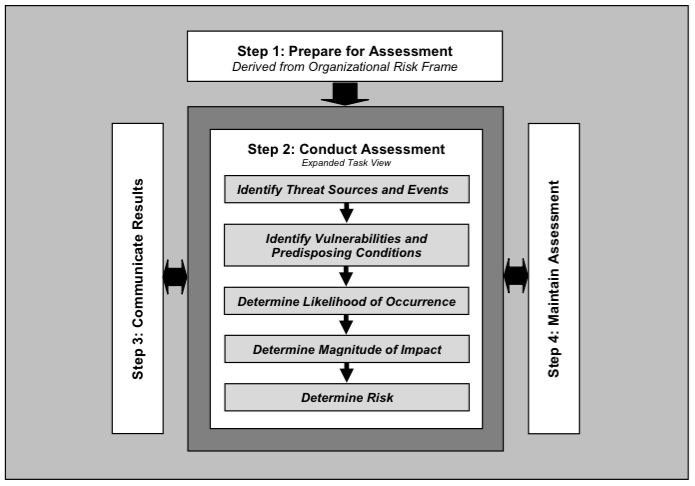
\includegraphics[scale=.55]{./img/RiskAssessmentProcess}
\caption{Risk Assessment Process (NIST Special Publication 800-30 Revision 1)}
\end{figure}
.\\
Define Threat Sources and Threat Events and determine Likelihoods and Impacts of Threat Events. Use the table below to rank and categorize risk.
\begin{figure}[h]
\centering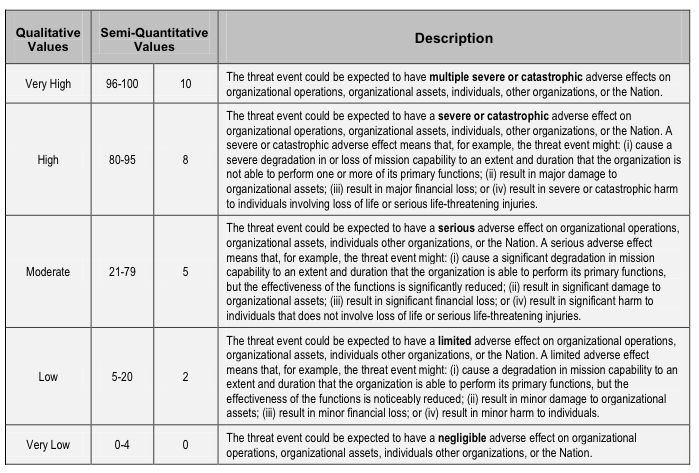
\includegraphics[scale=.55]{./img/QualitativeValues}
\caption{(Risk Values)}
\end{figure}
The formal Risk Assessment process is defined in NIST Special Publication 800-30 Revision 1. Read this document.\\\\
After completing a Risk Assessment, act on the results within the Risk Management Framework. You can respond to  risk and implment controls to midigate the risk or accept the risk and continue to monitor it.
\begin{figure}[h]
\centering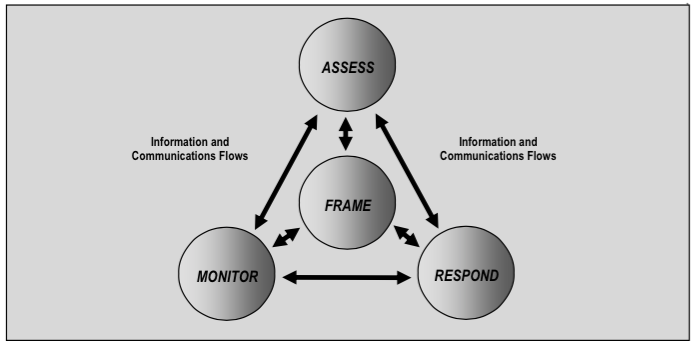
\includegraphics[scale=.55]{./img/RiskManagementProcess}
\caption{Risk Management Process (NIST Special Publication 800-39 \& NIST Special Publication 800-30 Revision 1)}
\end{figure}
\newpage
.
\newpage
.
\newpage
.
\subsubsection{Example Risk Assessment}
\begin{table}[h]\begin{center}\begin{tabular}{|p{1.9cm}|p{2.8cm}|p{1.3cm}|p{1.7cm}|p{1.3cm}|p{2.8cm}|p{1.4cm}|}\hline
Category & Risk & Impact & Likelihood & Risk Value & Mitigating Controls & Residual Risk\\\hline
Policy and Process & Visitor Policy allows visitors to walk around without escorts & Medium & Medium & Medium & Staff trained to keep sensitive information out-of-sight & Low\\\hline
Assessment & No Network Security Assessment allows gaps to go unnoticed & Medium & Medium & Medium & None & Medium\\\hline
Computer & Servers get infected with malware & High & Low & Medium & Anti-virus software & Low\\\hline
... & ... & ... & ... & ... & ... & ... \\\hline
\end{tabular}\end{center}\end{table}
\begin{equation}Risk\ Value = Impact * Likelihood\end{equation}
\begin{equation}Residual Risk = Risk Value - Mitigating\ Controls\end{equation}
\subsection{Gap Analyses}
A Gap Analysis is an assessment performed against an Information Security Standard to determines if the organization is in compliance with the standard. A Gap Analysis is common for any of the Laws, Regulations, and Standards mentioned in Policies and Processes. The product of the assessment lists the areas where the organization's Information Security Program meets the Law, Regulation, or Standard and areas where the organization needs to improve its Program.
\subsection{HIPAA Security Risk Analysis for Meaningful Use}
The HIPAA Security Rule requires all covered entities to annually "conduct an accurate and thorough assessment of the potential risks and vulnerabilities to the confidentiality, integrity, and availability of electronic protected health information held by the [organization]." This assessment is called a HIPAA Security Risk Analysis for Meaningful Use\resourcecite{SRA}\textsuperscript{,}\resourcecite{SRAGuidance}\textsuperscript{,}\resourcecite{SRAT}. It is really a Gap Analysis performed against the HIPAA Security Rule. NIST created a optional toolkit\resourcecite{HIPAATK} to assist in this assessment.
\subsection{Security Testing and Assessments (Offensive Security)}
Security Testing and Assessments incorporates all the activities you take to check every part of your Information Security Program. This is often called Offensive Security because the tester is 'attacking' your information. The rest of the topics in this book are defensive; you are protecting your information.\\\\
There is probably no other area of security that is more discussed or written about than Offensive Security. This section will be short because many other texts cover this section in tremendous depth. Overall, if it exists, you can test it, and you can probably break it.\\\\
Testing\resourcecite{NSA}\textsuperscript{,}\resourcecite{800115} usually follows a three step methodology of reconnaissance, enumeration, and exploitation. First, you locate what you are attacking, next you identify it, and last you break in. This could be accomplished by using nmap\resourcecite{nmap} to scan a netblock, using openvas\resourcecite{openvas} to identity a vulnerability, and using metasploit\resourcecite{metasploit} to exploit that vulnerability. All these tools are open source, but there are thousands of open source and commercial tools for Testing and Assessing.\\\\
Remember to use the System Model described in the beginning of this section to scope your testing and assessments. You may want to limit each engagement to only one network, computer, or application.\\\\
Use the output from your security testing and assessment program to create action. Create tickets for issues that need fixing. Create reports that trend how these programs are performing over time.
\subsubsection{Vulnerability Assessment and Management}
Vulnerability assessments attempt to locate all the vulnerable software on computers on your network. These tools typically have a list of vulnerabilities and attempt to look for each vulnerability on each computer. Your program should include vulnerability management to check the competency of the other parts of your program. However, do not base your patching process on vulnerability management. Vulnerability assessments\resourcecite{vulnpen} are limited to reconnaissance and enumeration.
\subsubsection{Penetration Testing}
Penetration Testing is a goals-driven assessment that attempts to compromise the Confidentiality, Integrity, or Availability of a system. These assessments go beyond reconnaissance and enumeration and exploit any discovered vulnerabilities. Penetration Testing is an essential component of your Risk Management Program. Internal penetration testing teams are called Red Teams while "defensive teams" are Blue Teams. Kali Linux\resourcecite{kali} is a distribution of Linux built for Penetration Testing.
\subsubsection{(Web/Mobile) Application Testing}
An application test, most common against web or mobile applications, is a penetration test limited to one single application. These tests are necessary to evaluate the security controls specific to that application. There are many tools\resourcecite{zap}\textsuperscript{,}\resourcecite{Nikto2}\textsuperscript{,}\resourcecite{Wnikto}\textsuperscript{,}\resourcecite{sqlmap}\textsuperscript{,}\resourcecite{skipfish}\textsuperscript{,}\resourcecite{burp}\textsuperscript{,}\resourcecite{firefoxaddons} and methodologies for these tests.\\
\subsubsection{Social Engineering}
Social Engineering is a test of your employees. These tests often try to trick employees over the phone/text, via email/message, or in person into compromising the Confidentiality, Integrity, or Availability of your information. While many executives do not believe in Social Engineering, these attacks are prevalent in the real world and responsible for many breaches. There are many tools\resourcecite{social}\textsuperscript{,}\resourcecite{phishing}\textsuperscript{,}\resourcecite{set} and methodologies for these tests.\\\\
Phishing is a social engineering attack against an entire company over. It is named because the attacker will cast their hook and lure and hope an employee bites. Spearphishing is a targeted phishing attack: the attacker researches a specific employee before launching the attack. Open Source Intelligence\resourcecite{WOSINT} (OSINT) refers to using information openly available on the Internet for Social Engineering attacks. There are many tools\resourcecite{Metagoofil}\textsuperscript{,}\resourcecite{SpiderFoot}\textsuperscript{,}\resourcecite{FOCA} available.
\subsubsection{Bug Bounty}
Bug Bounties are an external service or external or internal program that rewards researchers for finding bugs. These could be security bugs or other types of bugs. Reward internal employees for reporting bugs by giving them gift cards, t-shirts, etc. Reward your users for reporting bugs by paying them or giving them gift certificates. External services can also coordinate your bug bounty program with public or private researcher groups.\\\\
\textbf{Resources}
\begin{enumerate}
\resource[SecAssTypes]{Security Assessments Types}{https://danielmiessler.com/study/security-assessment-types/}
\resource[SRA]{Security Risk Assessment}{http://www.healthit.gov/security-risk-assessment}
\resource[SRAGuidance]{Guidance on Risk Analysis Requirements under the HIPAA Security Rule}{http://www.hhs.gov/ocr/privacy/hipaa/administrative/securityrule/rafinalguidancepdf.pdf}
\resource[HIPAATK]{HIPAA Security Rule Toolkit}{http://scap.nist.gov/hipaa/}
\resource[SRAT]{Security Risk Analysis Tipsheet}{http://www.cms.gov/Regulations-and-Guidance/Legislation/EHRIncentivePrograms/Downloads/SecurityRiskAssessment_FactSheet_Updated20131122.pdf}
\resource[NSA]{Network Security Assessment: Know Your Network (2nd Edition) By Chris McNab (2007)}{http://shop.oreilly.com/product/9780596006112.do}
\resource[800115]{Special Publication 800-115 Technical Guide to Information Security Testing and Assessment}{http://csrc.nist.gov/publications/nistpubs/800-115/SP800-115.pdf}
\resource[nmap]{nmap}{https://nmap.org}
\resource[openvas]{OpenVAS}{http://www.openvas.org}
\resource[metasploit]{Metasploit}{https://www.metasploit.com}
\resource[vulnpen]{The Difference Between a Vulnerability Assessment and a Penetration Test}{https://danielmiessler.com/essays/vulnerability_assessment_penetration_test/}
\resource[kali]{Kali Linux}{http://www.kali.org}
\resource[zap]{OWASP Zed Attack Proxy Project}{https://www.owasp.org/index.php/OWASP_Zed_Attack_Proxy_Project}
\resource[Nikto2]{Nikto2}{https://cirt.net/Nikto2}
\resource[Wnikto]{Nikto Web Scanner - Wikipedia}{https://en.wikipedia.org/wiki/Nikto_Web_Scanner}
\resource[sqlmap]{sqlmap}{http://sqlmap.org}
\resource[skipfish]{skipfish}{https://code.google.com/p/skipfish}
\resource[burp]{Burp Proxy}{http://portswigger.net/burp/proxy.html}
\resource[firefoxaddons]{Redspin Security Web Assesment Add-ons}{https://addons.mozilla.org/en-US/firefox/collections/nathan-drier/redspin-web/}
\resource[social]{An innovative and comprehensive framework for Social Vulnerability Assessment}{http://www.sicherheitsforschung-magdeburg.de/uploads/journal/MJS_033_Frumento_Assessment.pdf}
\resource[phishing]{Phishing Frenzy}{http://www.phishingfrenzy.com}
\resource[set]{Social Engineer Toolkit (SET)
}{http://www.social-engineer.org/framework/se-tools/computer-based/social-engineer-toolkit-set/}
\resource[WOSINT]{Open Source Intelligence - Wikipedia}{https://en.wikipedia.org/wiki/Open-source_intelligence}
\resource[Metagoofil]{Metagoofil}{http://www.edge-security.com/metagoofil.php}
\resource[SpiderFoot]{SpiderFoot}{http://www.spiderfoot.net/info/}
\resource[FOCA]{FOCA (Fingerprinting Organizations with Collected Archives)}{https://www.elevenpaths.com/labstools/foca/index.html}
\resource{Government Auditing Standards: 2011 Revision}{http://www.gao.gov/assets/590/587281.pdf}
\end{enumerate}